\documentclass[10pt]{article} % For LaTeX2e

% --- TMLR build mode -------------------------------------------------------
% Submission (double-blind, authors hidden). This is what TMLR requires.
\usepackage{tmlr}
% Camera-ready: swap the line above for the two below.
%\usepackage[accepted]{tmlr}
%\def\month{MM}\def\year{YYYY}\def\openreview{\url{https://openreview.net/forum?id=XXXX}}
% Preprint (de-anonymised, no TMLR branding):
%\usepackage[preprint]{tmlr}

% NOTE: math_commands.tex is deliberately NOT loaded. It redefines \eqref to
% print "equation N" instead of "(N)" and claims a very large macro namespace
% (\E, \R, \Tr, \Var, \KL, \1, ...). The template explicitly sanctions omitting
% it. We load amsmath ourselves instead.

\usepackage{amsmath}
\usepackage{amssymb}
\usepackage{amsthm}
\usepackage{booktabs}
\usepackage{multirow}
\usepackage{graphicx}
\usepackage{xcolor}
\usepackage{tikz}
\usetikzlibrary{arrows.meta,positioning,fit,backgrounds,calc}
\usepackage{algorithm}
\usepackage{algpseudocode}
\usepackage{hyperref}
\usepackage{url}
\usepackage[capitalise,noabbrev]{cleveref}

% --- palette used by the figures -------------------------------------------
\definecolor{hbmcol}{HTML}{C2410C}   % HBM-resident
\definecolor{regcol}{HTML}{0E7490}   % on-chip
\definecolor{predcol}{HTML}{6D28D9}  % model prediction

% --- notation --------------------------------------------------------------
\newcommand{\tX}{\mathsf{X}}
\newcommand{\tY}{\mathsf{Y}}
\newcommand{\tZ}{\mathsf{Z}}
\newcommand{\mW}{\mathbf{W}}
\newcommand{\mH}{\mathbf{H}}
\newcommand{\vs}{\mathbf{s}}
\newcommand{\Aop}{\mathcal{A}}          % Haar analysis
\newcommand{\Qio}{Q}                    % I/O cost
\newcommand{\dwconv}{\mathbin{\ast_{\mathrm{dw}}}}

\theoremstyle{plain}
\newtheorem{proposition}{Proposition}
\newtheorem{lemma}{Lemma}

\title{Wavelet Convolutions Are Memory-Bound:\\
       An I/O-Aware Formulation of {WTConv}}

% Authors are hidden by the tmlr package in submission mode. The block below
% is rendered only under [accepted] or [preprint].
\author{\name Anonymous Author \email anon@example.com \\
        \addr Anonymous Institution}

\begin{document}

\maketitle

\begin{abstract}
Wavelet convolution (WTConv) attains a receptive field that grows exponentially in the number of decomposition levels while its parameter count grows only linearly, and it drops into standard backbones without architectural change. Its reference implementation is nevertheless slower than the dense $7\times7$ convolution it is meant to replace, which has kept an asymptotically attractive operator practically unattractive. We show that this gap is not a constant-factor engineering artifact but a direct consequence of how the operator is expressed: WTConv performs $\mathcal{O}(1)$ arithmetic per element at an arithmetic intensity of $0.4$--$0.9$~FLOP/byte, roughly two orders of magnitude below the balance point of a modern GPU, so its cost is determined almost entirely by data movement between stages that each round-trip through high-bandwidth memory. We give an exact I/O-complexity accounting of the operator, deriving that the reference form moves $7N + \tfrac{43}{3}N(1-4^{-L})$ elements, i.e.\ $17.8$--$21.3N$, for an input of $N=B\cdot C\cdot H\cdot W$ elements and $L$ levels, against $2N$ of compulsory traffic, and we close most of that gap with four exact algebraic reformulations: the Haar analysis cascade is recomputed in registers at low arithmetic cost because the transform is multiplication-free; the $L$-level synthesis cascade collapses into a single closed-form pass whose sign pattern is indexed by the bits of the output coordinate, eliminating every intermediate low-pass plane; analysis, convolution and synthesis at the finest level collapse into one pass, which is a polyphase-structured full-resolution convolution whose sixteen phase pairs are generated from the $4k^2$ learned taps by a fixed orthogonal mixing, so that the largest intermediate in the layer is never written; and the learned per-channel scale is folded into the convolution weights by linearity. Because the normalised Haar matrix satisfies $\mathbf{H}=\mathbf{H}^{\!\top}=\mathbf{H}^{-1}$, analysis and synthesis exchange roles during backpropagation, so no separate derivative of the Haar transform is needed. The resulting formulation is a bit-exact reassociation of the original operator, not an approximation, and it moves $5N$ elements at $L{=}1$ and under $7.9N$ for any $L$, a $2.7$--$3.6\times$ reduction in traffic. Latency is a separate question, which we treat separately: a CUDA realisation measures $2.24$--$2.87\times$ in \texttt{fp32} and up to $3.84\times$ in \texttt{fp16}, at $1.5\times$ lower peak memory, with training curves indistinguishable from the reference. Because the argument is about data movement rather than any hardware feature, the same formulation transfers unchanged to Triton and to Apple Metal.
\end{abstract}

%==============================================================================
\section{Introduction}
%==============================================================================

Convolutional networks acquire large receptive fields slowly. Stacking $3\times3$ kernels grows the theoretical receptive field linearly in depth and the \emph{effective} receptive field only as $\mathcal{O}(\sqrt{n})$ \citep{luo2016erf}, which is a large part of why vision transformers, whose first layer already mixes globally \citep{dosovitskiy2021vit,liu2021swin}, were initially so competitive. The convolutional response has been to enlarge kernels directly: $31\times31$ re-parameterised depthwise kernels \citep{ding2022replknet}, or $51\times51$ sparse factorised ones \citep{liu2023slak}. Both buy receptive field at a parameter and FLOP cost that grows with the kernel area.

WTConv \citep{finder2024wavelet} takes a different route. It applies a small $k\times k$ depthwise kernel independently at each level of an $L$-level Haar decomposition. Because level $\ell$ operates on a $2^{\ell}$-times-downsampled grid, its footprint in input pixels is $k\cdot 2^{\ell}$, so an $L$-level layer reaches $k\cdot 2^{L}$ pixels using $\mathcal{O}(Lk^2C)$ parameters: the receptive field grows exponentially in $L$ while parameters grow linearly, i.e.\ parameters grow only logarithmically in the receptive field. It is a drop-in replacement for depthwise convolutions and improves accuracy and robustness in ConvNeXt and MobileNetV2 backbones \citep{liu2022convnext,sandler2018mobilenetv2}.

There is a catch that the asymptotics hide. In the reference implementation, a WTConv layer is \emph{slower than the dense $7\times7$ convolution it is supposed to replace}, by $1.14$--$1.65\times$ in our measurements. An operator that is cheaper in parameters and FLOPs but more expensive in wall-clock time is a poor trade in practice, and this is the gap we close.

\paragraph{The cost of WTConv is data movement, not arithmetic.}
Our starting observation is that WTConv is nowhere near compute-bound. Counting the multiply--accumulates the operator actually performs against the bytes its reference implementation actually moves gives an arithmetic intensity of $0.44$--$0.89$~FLOP/byte (\Cref{sec:memorybound}). An NVIDIA RTX~A6000 balances at roughly $50$~FLOP/byte. The operator therefore sits two orders of magnitude to the left of the roofline ridge: the GPU spends essentially all of its time waiting for memory, and the arithmetic, including the Haar transform itself, is free in comparison. This reframes the problem. The question is not how to compute the wavelet transform faster; it is how to stop writing intermediate tensors to high-bandwidth memory (HBM). The same reframing drove FlashAttention \citep{dao2022flashattention}, and the analogy is close: in both cases a mathematically elegant operator was expressed as a chain of memory-bound primitives, and in both cases the fix is a reassociation that keeps intermediates on chip.

\paragraph{What makes WTConv especially amenable.}
Two structural properties of the Haar basis make the reassociation unusually clean, and they are what we exploit.

\emph{Haar analysis has low arithmetic cost.} The $2\times2$ transform uses only sums, differences, and fixed scaling by $\tfrac12$. Recomputing its coefficients is therefore inexpensive compared with storing and reloading them. Longer wavelet filters would make this trade-off less favourable.

\emph{The normalised Haar operator is symmetric and self-inverse.} With the $\tfrac12$ normalisation, the $4\times4$ analysis matrix satisfies $\mH=\mH^{\!\top}=\mH^{-1}$ exactly (\Cref{prop:selfinverse}). Consequently, analysis and synthesis exchange roles during backpropagation, and no separate derivative of the Haar transform is needed.

\paragraph{Contributions.}
\begin{itemize}\itemsep2pt
\item \textbf{A cost model for WTConv} (\Cref{sec:memorybound}). We give a closed form for the operator that eliminates the recursive low-pass carrier, and an exact element-by-element I/O accounting of the reference implementation: $\Qio_{\mathrm{ref}} = 7N + \tfrac{43}{3}N(1-4^{-L})$. We place the operator on the roofline and show it is bandwidth-bound by two orders of magnitude.
\item \textbf{An I/O-reduced reformulation} (\Cref{sec:method}) built from four exact algebraic identities (register-resident analysis, closed-form single-pass synthesis, end-to-end collapse of the finest level, and scale folding), reaching $5N$ at $L{=}1$ and at most $\tfrac{47}{6}N$ for any $L$, against $2N$ of compulsory traffic --- a $3.55\times$ reduction at $L{=}1$ falling to $\tfrac{128}{47}\approx2.72\times$ as $L$ grows. Two steps are algorithmic rather than mechanical. The synthesis collapse (\Cref{sec:synthesis}) turns an $L$-level inverse cascade, normally $L$ dependent passes, into one pass whose per-level sign pattern is read off the bits of the output coordinate. The level collapse (\Cref{sec:levelcollapse}) fuses analysis, convolution and synthesis into a single polyphase-structured convolution, which removes the layer's largest intermediate; we show why that structure should be kept factored rather than materialised as a $2k\times2k$ kernel.
\item \textbf{Measurement} (\Cref{sec:experiments}). A CUDA realisation measures $2.24$--$2.87\times$ in \texttt{fp32} and up to $3.84\times$ in \texttt{fp16}, at $1.5\times$ lower peak memory. We report traffic and latency separately and do not claim a proportionality between them (\Cref{sec:prediction}).
\item \textbf{Exactness, not approximation.} Every step is a reassociation of the same multilinear map, so agreement with the reference is limited only by floating-point reassociation error, which we quantify for the forward pass and for every gradient the layer produces.
\end{itemize}

We develop the argument for a single CUDA realisation to keep the exposition concrete. Because the reformulation is about data movement and not about any hardware feature, it transfers unchanged; we summarise Triton and Apple~Metal realisations in \Cref{sec:portability} and \Cref{app:backends}.

%==============================================================================
\section{Background}
\label{sec:background}
%==============================================================================

\subsection{The WTConv operator}

Let $\tX\in\mathbb{R}^{B\times C\times H\times W}$ denote the input, and let $N=B\cdot C\cdot H\cdot W$ be its element count, the unit in which we quote every I/O cost. Let $\dwconv$ denote depthwise convolution (one $k\times k$ kernel per channel, zero-padded to preserve resolution) and let $\odot$ denote per-channel scaling.

Let $\Aop$ denote one level of Haar analysis, which splits each channel into four half-resolution subbands $(\mathrm{LL},\mathrm{LH},\mathrm{HL},\mathrm{HH})$, and let $\Aop^{\!\top}$ denote its synthesis, which inverts it exactly (\Cref{prop:selfinverse}). For a tensor carrying a subband axis, let $[\,\cdot\,]_{\mathrm{LL}}$ denote the low-pass band, $[\,\cdot\,]_{\mathrm{H}}$ the three high-pass bands, and $\Vert$ their concatenation. WTConv preserves the channel count. It learns a $k\times k$ kernel and a per-channel scale at each level, $(\mW^{(\ell)},\vs^{(\ell)})$ for $\ell=1,\dots,L$, together with a full-resolution base convolution $(\mW^{(0)},b,\vs^{(0)})$, giving $\mathcal{O}(Lk^2C)$ parameters in total. \Cref{alg:wtconv} states the operator as the reference implements it.

\begin{algorithm}[!ht]
\caption{WTConv, reference form \citep{finder2024wavelet}}
\label{alg:wtconv}
\begin{algorithmic}[1]
\Require input $\tX$, levels $L$, parameters $\{\mW^{(\ell)},\vs^{(\ell)}\}_{\ell=0}^{L}$, bias $b$
\State $\tX^{(0)} \gets \tX$ \Comment{decomposition carrier}
\For{$\ell = 1,\dots,L$} \Comment{downward: decompose and filter}
  \State $\tY^{(\ell)} \gets \Aop\,\tX^{(\ell-1)}$ \Comment{Haar analysis}
  \State $\tZ^{(\ell)} \gets \vs^{(\ell)}\odot\bigl(\tY^{(\ell)}\dwconv\mW^{(\ell)}\bigr)$ \Comment{filter, then scale}
  \State $\tX^{(\ell)} \gets \bigl[\tY^{(\ell)}\bigr]_{\mathrm{LL}}$ \Comment{carry the \emph{raw}, unfiltered low-pass band}
\EndFor
\State $R^{(L+1)} \gets 0$
\For{$\ell = L,\dots,1$} \Comment{upward: reconstruct and accumulate}
  \State $R^{(\ell)} \gets \Aop^{\!\top}\Bigl(\bigl(\bigl[\tZ^{(\ell)}\bigr]_{\mathrm{LL}} + R^{(\ell+1)}\bigr)\ \Big\Vert\ \bigl[\tZ^{(\ell)}\bigr]_{\mathrm{H}}\Bigr)$
\EndFor
\State \Return $\vs^{(0)}\odot\bigl(\tX\dwconv\mW^{(0)} + b\bigr) + R^{(1)}$ \Comment{base path $+$ reconstruction}
\end{algorithmic}
\end{algorithm}

\subsection{Haar transform differentiation}
\label{sec:haar-backprop}

For each non-overlapping $2\times2$ block, the normalised Haar transform maps
four input samples to four subband coefficients using the following matrix.

\begin{proposition}[Symmetry and self-inversion]
\label{prop:selfinverse}
$\mH=\tfrac12\left[\begin{smallmatrix}1&1&1&1\\1&1&-1&-1\\1&-1&1&-1\\1&-1&-1&1\end{smallmatrix}\right]$
satisfies $\mH^{\!\top}=\mH$ and $\mH^2=\mathbf{I}$. Therefore,
$\mH^{-1}=\mH^{\!\top}=\mH$.
\end{proposition}

The full analysis operator $\Aop$ applies $\mH$ independently to every block,
and synthesis applies $\Aop^{\!\top}$. For $\mathbf{y}=\mH\mathbf{x}$, the
chain rule gives
\begin{equation}
\frac{\partial\mathcal{L}}{\partial\mathbf{x}}
= \mH^{\!\top}\frac{\partial\mathcal{L}}{\partial\mathbf{y}}
= \mH\frac{\partial\mathcal{L}}{\partial\mathbf{y}}.
\end{equation}
Thus, backward through analysis applies synthesis, and backward through
synthesis applies analysis. The Haar step needs no separate derivative;
convolution and scale gradients are computed as usual.


\subsection{The roofline}
\label{roofline}

The roofline model \citep{williams2009roofline} bounds attainable throughput by $\min(\pi,\, \beta I)$ where $\pi$ is peak compute, $\beta$ peak bandwidth, and $I$ the arithmetic intensity in FLOP/byte. The ridge point $I^\star=\pi/\beta$ separates memory-bound from compute-bound operation. For the RTX~A6000 used throughout, $\beta=768$~GB/s and $\pi\approx38.7$~TFLOP/s in \texttt{fp32}, so $I^\star\approx50$~FLOP/byte. Any operator with $I\ll I^\star$ is bandwidth-limited: its runtime is governed by the bytes it moves rather than by how the arithmetic is scheduled. The bound is an upper bound on attainable throughput and not an equality, so this identifies traffic as the quantity to minimise without implying that runtime is proportional to it. The practical content of this paper is that WTConv is deeply in that regime, so minimising traffic is not merely one optimisation among many: it is the whole problem.


\clearpage
%==============================================================================
\section{WTConv is memory-bound}
\label{sec:memorybound}
%==============================================================================

\subsection{I/O cost of the reference implementation}

The reference implementation expresses each level as a chain of framework primitives, every one of which reads its input from HBM and writes its output back (\Cref{fig:dataflow}a). We count elements crossing the HBM boundary: each stage reads its input tensor once and writes its output tensor once, weight traffic is $\mathcal{O}(Ck^2)$ and therefore negligible against $\mathcal{O}(N)$. Writing $N_\ell = N/4^{\ell-1}$ for the element count entering level $\ell$:


\begin{itemize}\itemsep1pt
\item \emph{Analysis}, per level: the Haar transform is executed as a grouped stride-2 \texttt{conv2d} against a constant $\pm\tfrac12$ filter ($2N_\ell$); the depthwise convolution over the $4C$-channel coefficient tensor ($2N_\ell$); the scale multiply ($2N_\ell$). Total $6N_\ell$.
\item \emph{Synthesis}, per level: the cross-level low-pass add ($\tfrac34 N_\ell$); the concatenation of the summed low-pass band with the three high bands ($2N_\ell$); the \texttt{conv\_transpose2d} ($2N_\ell$). Total $\tfrac{19}{4}N_\ell$.
\item \emph{Base path}: convolution ($2N$), scale multiply ($2N$), final add ($3N$). Total $7N$.
\end{itemize}

Using $\sum_{\ell=1}^{L}4^{-(\ell-1)}=\tfrac43(1-4^{-L})$,
\begin{equation}
\Qio_{\mathrm{ref}} \;=\; 7N \;+\; \Bigl(6+\tfrac{19}{4}\Bigr)\cdot\tfrac43\,N\bigl(1-4^{-L}\bigr)
\;=\; 7N + \tfrac{43}{3}\,N\bigl(1-4^{-L}\bigr),
\label{eq:qref}
\end{equation}
rising from $17.75N$ at $L=1$ to $21.33N$ as $L\to\infty$; that is, evaluating the layer moves between $18$ and $21$ times the input tensor's worth of data through HBM. For a representative $B{=}8$, $C{=}64$, $H{=}W{=}256$ input, $N=33.6$M elements ($128$\,MiB in \texttt{fp32}) and the reference therefore moves roughly $2.9$\,GB per forward pass.

\subsection{Arithmetic intensity of the reference implementation}

 The base convolution performs $k^2$ multiply--accumulates per element. At level $\ell$, the depthwise convolution over the coefficient tensor costs a further $k^2$ per element of $N_\ell$, and the analysis and synthesis each cost $4$, since the reference executes both as $2\times2$ convolutions rather than as additions. Summing over levels with the same geometric factor as before,
\begin{equation}
\mathrm{MAC} \;=\; N\bigl[k^2 + (k^2+8)\cdot\tfrac43\bigl(1-4^{-L}\bigr)\bigr].
\label{eq:mac}
\end{equation}
For $k=3$ and $L=5$ this is $31.6N$ multiply--accumulates, or $63.3N$ FLOPs, against $4\Qio_{\mathrm{ref}}=85.3N$ bytes in \texttt{fp32}:
\begin{equation}
I_{\mathrm{ref}} \;=\; \frac{63.3N}{85.3N} \;\approx\; 0.74~\text{FLOP/byte}.
\label{eq:intensity}
\end{equation}
 Against the ridge point $I^\star\approx50$ (\autoref{roofline}), WTConv therefore sits almost $70\times$ to the left of the ridge (\Cref{fig:roofline}), using under $2\%$ of the machine's arithmetic capability. The arithmetic is not the problem: no amount of faster transform evaluation would help, and only removing traffic can.



\begin{figure}[t]
\centering
% Figure: HBM dataflow of a single WTConv level, baseline vs. fused.
% Requires: tikz + libraries arrows.meta, positioning, fit, backgrounds, calc
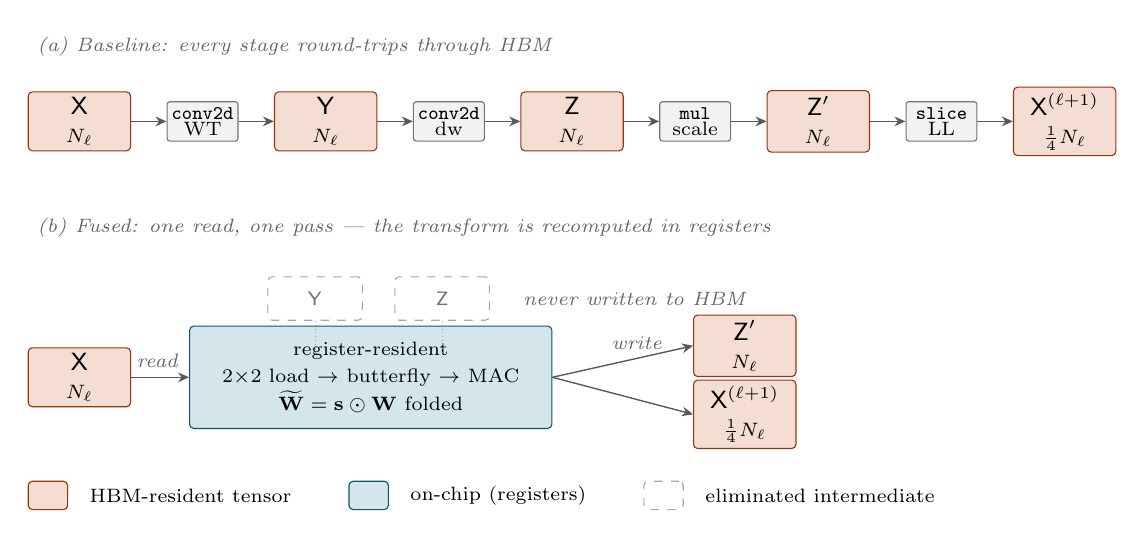
\begin{tikzpicture}[
  font=\small,
  node distance=0pt,
  hbm/.style={draw=hbmcol!80!black, fill=hbmcol!18, rounded corners=1.5pt,
              minimum height=6.5mm, minimum width=13mm, align=center, inner sep=2pt},
  reg/.style={draw=regcol!75!black, fill=regcol!18, rounded corners=1.5pt,
              minimum height=6.5mm, minimum width=13mm, align=center, inner sep=2pt},
  op/.style={draw=black!55, fill=black!5, rounded corners=1pt,
             minimum height=5mm, minimum width=9mm, align=center, inner sep=1.5pt,
             font=\scriptsize},
  flow/.style={-{Stealth[length=4pt,width=3.5pt]}, draw=black!65, line width=0.5pt},
  ghost/.style={draw=black!35, dashed, fill=none, rounded corners=1.5pt,
                minimum height=5.5mm, minimum width=12mm, align=center, inner sep=2pt,
                font=\scriptsize, text=black!55},
  lbl/.style={font=\scriptsize\itshape, text=black!60},
]

%============================ (a) BASELINE ============================
\node[lbl, anchor=west] at (0,0.95) {(a) Baseline: every stage round-trips through HBM};

\node[hbm, anchor=west] (b0) at (0,0) {$\tX$\\[-1pt]\scriptsize $N_\ell$};
\node[op,  right=4.5mm of b0]   (bop1) {\texttt{conv2d}\\[-2pt]\scriptsize WT};
\node[hbm, right=4.5mm of bop1] (b1)   {$\tY$\\[-1pt]\scriptsize $N_\ell$};
\node[op,  right=4.5mm of b1]   (bop2) {\texttt{conv2d}\\[-2pt]\scriptsize dw};
\node[hbm, right=4.5mm of bop2] (b2)   {$\tZ$\\[-1pt]\scriptsize $N_\ell$};
\node[op,  right=4.5mm of b2]   (bop3) {\texttt{mul}\\[-2pt]\scriptsize scale};
\node[hbm, right=4.5mm of bop3] (b3)   {$\tZ'$\\[-1pt]\scriptsize $N_\ell$};
\node[op,  right=4.5mm of b3]   (bop4) {\texttt{slice}\\[-2pt]\scriptsize LL};
\node[hbm, right=4.5mm of bop4] (b4)   {$\tX^{(\ell+1)}$\\[-1pt]\scriptsize $\tfrac{1}{4}N_\ell$};

\foreach \a/\b in {b0/bop1, bop1/b1, b1/bop2, bop2/b2, b2/bop3, bop3/b3, b3/bop4, bop4/b4}
  \draw[flow] (\a) -- (\b);

%============================ (b) FUSED ============================
\node[lbl, anchor=west] at (0,-1.35) {(b) Fused: one read, one pass --- the transform is recomputed in registers};

% ghosts: intermediates that are never materialised
\node[ghost] (g1) at (3.65,-2.25) {$\tY$};
\node[ghost, right=4mm of g1] (g2) {$\tZ$};
\node[lbl, right=3mm of g2] {never written to HBM};

\node[hbm, anchor=west] (f0) at (0,-3.25) {$\tX$\\[-1pt]\scriptsize $N_\ell$};

\node[reg, anchor=west, minimum width=46mm, minimum height=13mm] (freg) at (2.05,-3.25)
  {\scriptsize register-resident\\[-1pt]\scriptsize
   $2{\times}2$ load $\to$ butterfly $\to$ MAC\\[-1pt]\scriptsize
   $\widetilde{\mW}=\vs\odot\mW$ folded};

\node[hbm, anchor=west] (f3) at (8.45,-2.85) {$\tZ'$\\[-1pt]\scriptsize $N_\ell$};
\node[hbm, anchor=west] (f4) at (8.45,-3.72) {$\tX^{(\ell+1)}$\\[-1pt]\scriptsize $\tfrac{1}{4}N_\ell$};

\draw[flow] (f0) -- node[lbl, above, pos=0.45] {read} (freg);
\draw[flow] (freg.east) -- node[lbl, above, pos=0.6, yshift=-0.5pt] {write} (f3.west);
\draw[flow] (freg.east) -- (f4.west);

\draw[densely dotted, draw=black!35] (g1.south) -- ++(0,-4mm);
\draw[densely dotted, draw=black!35] (g2.south) -- ++(0,-4mm);

%============================ LEGEND ============================
\begin{scope}[shift={(0,-4.75)}]
  \node[hbm, minimum width=5mm, minimum height=3.6mm, anchor=west] (lg1) at (0,0) {};
  \node[anchor=west, font=\scriptsize, right=1.5mm of lg1] (lt1) {HBM-resident tensor};
  \node[reg, minimum width=5mm, minimum height=3.6mm, anchor=west, right=6mm of lt1] (lg2) {};
  \node[anchor=west, font=\scriptsize, right=1.5mm of lg2] (lt2) {on-chip (registers)};
  \node[ghost, minimum width=5mm, minimum height=3.6mm, anchor=west, right=6mm of lt2] (lg3) {};
  \node[anchor=west, font=\scriptsize, right=1.5mm of lg3] {eliminated intermediate};
\end{scope}

\end{tikzpicture}

\caption{HBM dataflow for one WTConv decomposition level $\ell$, with $N_\ell = N/4^{\ell-1}$ the number of elements entering that level. (a)~The reference implementation expresses the level as a chain of framework primitives; every stage materialises a full-size tensor in HBM, so the level costs $6N_\ell$ of traffic. (b)~The fused formulation reads the input once, evaluates the Haar butterfly and the depthwise convolution in registers against weights that already carry the learned scale, and writes only the results that later stages genuinely need, for $\tfrac94 N_\ell$. $\tY$ and $\tZ$ are never written. This is the form used at levels $\ell\ge2$; at $\ell=1$ the synthesis is absorbed as well (\Cref{sec:levelcollapse}), so not even the filtered coefficients are written.}
\label{fig:dataflow}
\end{figure}

%==============================================================================
\section{An I/O-Aware formulation}
\label{sec:method}
%==============================================================================

We reduce the I/O cost in \Cref{eq:qref} through four algebraically equivalent
reformulations. They preserve the operator in exact arithmetic and differ from
the reference only in floating-point evaluation order.

\subsection{Register-resident Haar analysis}
\label{sec:analysis}

For a $2\times2$ patch $[[a,b],[c,d]]$, the normalised Haar analysis is
\begin{equation}
\begin{aligned}
\mathrm{LL} &= \tfrac12(a+b+c+d), &\qquad \mathrm{LH} &= \tfrac12(a+b-c-d),\\
\mathrm{HL} &= \tfrac12(a-b+c-d), &\qquad \mathrm{HH} &= \tfrac12(a-b-c+d),
\end{aligned}
\label{eq:butterfly}
\end{equation}
They can be computed by first forming
$\sigma_{ac}=a+c,\ \delta_{ac}=a-c,\ \sigma_{bd}=b+d,$ and
$\delta_{bd}=b-d$, followed by four pairwise combinations. This requires eight
additions and four halvings, with no general multiplication. The reference
implementation instead evaluates \Cref{eq:butterfly} as a grouped convolution
with fixed $\pm\tfrac12$ filters.

WTConv has an arithmetic intensity of approximately $0.74$~FLOP/byte, so data
movement dominates its runtime. We therefore compute the Haar coefficients
inside the depthwise-convolution kernel instead of materialising them in HBM.
For output position $(h',w')$ and convolution tap $(\kappa_h,\kappa_w)$, the
kernel reads the $2\times2$ input block beginning at
\begin{equation*}
i_h = 2h' + 2\kappa_h - (k-1), \qquad
i_w = 2w' + 2\kappa_w - (k-1).
\end{equation*}
It forms the four coefficients of \Cref{eq:butterfly} in registers and
immediately accumulates them into the four convolution outputs. The
intermediate coefficient tensor $\tY$ is never written.

Each block stages the partial sums for its output tile, together with a $k-1$
halo, in shared memory, so an input element is fetched once per tile rather than
once per tap; halo elements are fetched by the neighbouring tile as well and are
served from L2.

A level that publishes its coefficients therefore reads $N_\ell$ input elements,
writes $N_\ell$ filtered coefficients for synthesis, and writes
$\tfrac14N_\ell$ raw low-pass coefficients for the next level: $\tfrac94N_\ell$
in total, against $6N_\ell$ for the reference. The deepest level feeds no
successor and writes $2N_\ell$. Level~1 publishes nothing at all, for the reason
given in \Cref{sec:levelcollapse}.

\subsection{Collapsing the synthesis cascade}
\label{sec:synthesis}

The analysis above still leaves the upward loop of \Cref{alg:wtconv}: a sequential recursion of $L$ steps, each reading the level below, adding, concatenating, and expanding. Executed literally it costs $\tfrac{19}{4}N_\ell$ per level and, worse, serialises the levels.

The recursion can be eliminated. The low-pass carrier is the only coupling between levels and it enters linearly, so the levels superpose: the contribution of \emph{any} level to \emph{any} output pixel is a signed constant multiple of one of its coefficients. Haar synthesis at level $\ell$ replicates each coefficient over a $2^{\ell}$ block with a sign pattern, and which sign applies is determined by the position of the output pixel within that block; that is, by the low bits of its coordinates.

\begin{proposition}[Bit-indexed synthesis]
\label{prop:bitindexed}
Let $(y,x)$ index an output pixel and let level $\ell$ have coefficients $c^{(\ell)}_{\mathrm{LL}},c^{(\ell)}_{\mathrm{LH}},c^{(\ell)}_{\mathrm{HL}},c^{(\ell)}_{\mathrm{HH}}$ at coarse position $(y\gg\ell,\,x\gg\ell)$. Write $q_y^{(\ell)} = (y \gg (\ell-1))\,\&\,1$ and $q_x^{(\ell)} = (x \gg (\ell-1))\,\&\,1$. Then the total synthesis at $(y,x)$ is
\begin{equation}
R_{y,x} \;=\; \sum_{\ell=1}^{L} 2^{-\ell}\Bigl(
 c^{(\ell)}_{\mathrm{LL}}
 + (-1)^{q_y^{(\ell)}} c^{(\ell)}_{\mathrm{LH}}
 + (-1)^{q_x^{(\ell)}} c^{(\ell)}_{\mathrm{HL}}
 + (-1)^{q_y^{(\ell)}\oplus q_x^{(\ell)}} c^{(\ell)}_{\mathrm{HH}}\Bigr),
\end{equation}
where the low-pass terms telescope through the cascade.
\end{proposition}

The practical consequence is that the entire reconstruction, together with the cross-level accumulation, becomes \emph{one} pass: each thread walks the levels from the deepest upward, addressing its ancestor coefficient by a shift and selecting signs by a parity test, and writes its finished pixels once. No intermediate low-pass plane is ever materialised, and the $L$ sequential dependencies disappear. Coarse-level coefficients are re-read by many threads, but they are small ($4^{-\ell}$ of the tensor) and served from cache; this is the same recompute-instead-of-communicate exchange as \Cref{sec:analysis}, applied to communication between levels rather than between stages.

In the formulation we settle on, this pass covers levels $2,\dots,L$ and lands on level~1's coefficient grid rather than on the output, because level~1's synthesis is absorbed into its analysis kernel by the next identity. It therefore reads $\sum_{\ell\ge2}N_\ell$ and writes $\tfrac14N$.

\subsection{Collapsing a level end to end}
\label{sec:levelcollapse}

Analysis and synthesis can be fused with the convolution between them, not only
with the stages on one side of it. Substituting the tap loop of
\Cref{sec:analysis} into the synthesis of \Cref{sec:synthesis} at one level, and
writing $R$ for that level's contribution to the output, gives for each output
phase $(q_y,q_x)\in\{0,1\}^2$
\begin{equation}
R_{2h+q_y,\,2w+q_x}
=\sum_{\kappa_h,\kappa_w}\ \sum_{r_y,r_x\in\{0,1\}}
  \Omega^{(q_y,q_x)}_{(r_y,r_x)}[\kappa_h,\kappa_w]\;
  \tX\bigl[2h+2\kappa_h-(k-1)+r_y,\ \ 2w+2\kappa_w-(k-1)+r_x\bigr],
\label{eq:polyphase}
\end{equation}
addressing the input exactly as in \Cref{sec:analysis}, with
\begin{equation}
\Omega^{(q_y,q_x)}_{(r_y,r_x)}[\kappa_h,\kappa_w]
=\sum_{s}\ \mH\bigl[s,(q_y,q_x)\bigr]\ \mH\bigl[s,(r_y,r_x)\bigr]\
  \widetilde{\mW}_s[\kappa_h,\kappa_w],
\label{eq:omega}
\end{equation}
the sum running over the four subbands. A WTConv level is therefore a
polyphase-structured full-resolution depthwise convolution: a $2k\times2k$
kernel whose sixteen phase pairs are all generated from the $4k^2$ learned taps
by a fixed orthogonal mixing.

The structure must not be materialised. Forming $\Omega$ and calling a
$2k\times2k$ depthwise convolution would quadruple both the
multiply--accumulates and the weight traffic, and it could not express the
cross-level term at all. Kept factored --- partial sums, $k^2$ taps, then the
butterfly --- synthesis is pointwise within the $2\times2$ block a thread
already owns: no halo, no extra taps, four butterflies per output block. It is
free in arithmetic, and its entire effect is on traffic. At level~1 the
coefficient tensor $\tZ$, the largest intermediate in the layer, is never
written and never read back; the cross-level term of \Cref{alg:wtconv} is added
into the low-pass accumulator before the butterfly, and the base-path addition
folds into the same store.

One dependency stops us applying this at every level simultaneously. Level
$\ell+1$ consumes the \emph{raw} low-pass band of level $\ell$, while the
synthesis at level $\ell$ consumes the reconstruction of level $\ell+1$; fusing
analysis and synthesis at level $\ell$ closes that cycle. We break it at
level~1 only, by computing its raw low-pass band in a separate pass that applies
just the first row of $\mH$ ($N$ read, $\tfrac14N$ written), and leaving levels
$2,\dots,L$ in the published-coefficient form of \Cref{sec:analysis}. Those
levels carry a quarter of the work of their predecessor, so the extra pass buys
the collapse where the tensors are largest.

\subsection{Folding the learned scale}

The per-channel scale is applied after the convolution, $\tZ_c = s_c\,(\tX\dwconv\mW)_c$: a pure elementwise pass at intensity $\tfrac14$~FLOP/byte, i.e.\ the single most bandwidth-inefficient stage in the layer. By linearity of convolution it need not exist at all. Defining $\widetilde{\mW}_c = s_c\mW_c$ gives $\tZ = \tX\dwconv\widetilde{\mW}$ exactly, and the fold costs $\mathcal{O}(Ck^2)$, negligible against $\mathcal{O}(N)$. In the base path this lets us keep using the vendor convolution, which is difficult to beat, while removing the scale pass entirely; in the wavelet path the folded weights are what the register-resident kernel consumes.

The fold must be carried through the backward pass, which is where it is easy to go wrong: since $\widetilde{\mW}=\vs\odot\mW$,
\begin{equation}
\frac{\partial\mathcal{L}}{\partial\mW_c} = s_c\,\frac{\partial\mathcal{L}}{\partial\widetilde{\mW}_c},
\qquad
\frac{\partial\mathcal{L}}{\partial s_c} = \Bigl\langle \frac{\partial\mathcal{L}}{\partial\widetilde{\mW}_c},\, \mW_c \Bigr\rangle .
\label{eq:foldgrad}
\end{equation}
Omitting the factor $s_c$ in the first identity yields a weight gradient that is wrong by a per-channel constant; and, because the scale is initialised to $1$, one that is correct at initialisation and silently degrades as training proceeds. We flag this because we found exactly this error in our own base-path implementation while preparing the equivalence tests of \Cref{sec:equivalence}; the tests in this paper are what caught it.

\subsection{The resulting I/O cost}
\label{sec:prediction}

Collecting the four reformulations, with $N_\ell = N/4^{\ell-1}$ as before:
\begin{itemize}\itemsep1pt
\item \emph{Base path}: the folded vendor convolution reads $N$ and writes $N$.
\item \emph{Low-pass pass} (only when $L\ge2$): $N$ read, $\tfrac14N$ written.
\item \emph{Analysis}, levels $2\le\ell\le L$: $\tfrac94N_\ell$ each, less the $\tfrac14N_L$ the deepest level does not write.
\item \emph{Synthesis} of levels $2,\dots,L$: reads $\sum_{\ell\ge2}N_\ell$, writes $\tfrac14N$.
\item \emph{Fused level~1}: reads $N$ (input), $\tfrac14N$ (the deeper reconstruction, absent at $L=1$) and $N$ (base path); writes $N$.
\end{itemize}
Using $\sum_{\ell=2}^{L}N_\ell=\tfrac13N\bigl(1-4^{1-L}\bigr)$,
\begin{equation}
\Qio_{\mathrm{fused}} \;=\;
\begin{cases}
5N, & L=1,\\[4pt]
\tfrac{47}{6}N \;-\; \tfrac43 N\,4^{\,1-L}, & L\ge2,
\end{cases}
\label{eq:qfused}
\end{equation}
that is $5.00N,\,7.50N,\,7.75N,\,7.81N,\,7.83N$ for $L=1,\dots,5$, against
$\Qio_{\mathrm{ref}} = 17.75N,\,20.44N,\,21.11N,\,21.28N,\,21.32N$ from
\Cref{eq:qref}. The compulsory traffic (read the input, write the output) is
$2N$: the fused form stays within $2.5$--$3.9\times$ of it where the reference is
within $8.9$--$10.7\times$.

\begin{table}[h]
\centering
\caption{Elements crossing the HBM boundary per forward evaluation, in units of $N=B\cdot C\cdot H\cdot W$, from \Cref{eq:qref} and \Cref{eq:qfused}. The last row is a ratio of \emph{traffic}, not of runtime; see the discussion below.}
\label{tab:traffic}
\begin{tabular}{lccccc}
\toprule
& \multicolumn{5}{c}{Decomposition levels $L$}\\
\cmidrule(lr){2-6}
 & 1 & 2 & 3 & 4 & 5 \\
\midrule
Reference, $\Qio_{\mathrm{ref}}$ & $17.75N$ & $20.44N$ & $21.11N$ & $21.28N$ & $21.32N$ \\
Fused, $\Qio_{\mathrm{fused}}$   & $5.00N$  & $7.50N$  & $7.75N$  & $7.81N$  & $7.83N$ \\
\addlinespace[2pt]
Traffic removed & $3.55\times$ & $2.73\times$ & $2.72\times$ & $2.72\times$ & $2.72\times$ \\
\bottomrule
\end{tabular}
\end{table}

\Cref{tab:traffic} gives the reduction level by level. It is sharpest at $L=1$,
exactly $\tfrac{71}{20}=3.55$, because a single-level layer is absorbed entirely
by \Cref{sec:levelcollapse}: there is no low-pass pass and no cascade to pay for,
and the layer degenerates to the base convolution plus one kernel that reads the
input and writes the output. Beyond that the ratio drops and then flattens,
tending to $\tfrac{128}{47}\approx2.72$, and the two effects responsible are
worth separating. Deeper levels must publish their coefficients for the cascade
to consume, so they keep the $\tfrac94N_\ell$ form rather than the collapsed one;
and breaking the analysis--synthesis cycle at level~1 costs an extra full read of
the input for the low-pass pass. Both charges are levied once, against a
geometric series that has already converged by $L=3$, which is why the ratio is
essentially constant from there on. The reference's own traffic saturates for the
same reason, at $\tfrac{64}{3}N$.

\paragraph{Traffic is not latency.}
Both forms sit far to the left of the ridge point, which is what makes traffic
the quantity worth minimising and what explains the direction of the result. The
last row of \Cref{tab:traffic} is nevertheless a statement about elements moved
and nothing more; we do not read it as a predicted speedup. The map from elements
counted to seconds elapsed is not a proportionality, and the discrepancies do not
all pull the same way: not every counted element reaches
DRAM, since halo elements and coarse-level coefficients are re-read from L2 and
the two forms differ in how much of their traffic is cacheable; the two forms
issue different numbers of kernels ($5L+\mathcal{O}(1)$ launches against at most
three), so per-launch overhead and tail effects are weighted differently; the
base convolution is a vendor kernel in both arms and does not scale with the
fusion at all; and achieved bandwidth is itself a function of access pattern and
occupancy, which the two forms do not share. A ratio of counted elements is
moreover dtype-independent by construction, while the measured ratios are not
(\Cref{sec:speed}) --- direct evidence that the mapping is not proportional. We
therefore report traffic as traffic and latency as latency, and claim only that
the former is the mechanism behind the latter.

\begin{figure}[t]
\centering
% Roofline for the RTX A6000. Hand-placed log-log coordinates so the figure has
% no pgfplots dependency.
%   X(I) = 2.6*(log10(I)+1)      I in FLOP/byte,  domain 1e-1 .. 1e3
%   Y(P) = 1.7*(log10(P)-2)      P in GFLOP/s,    domain 1e2  .. 1e5
% beta = 768 GB/s, pi = 38.7 TFLOP/s, ridge I* = 50.4 FLOP/byte.
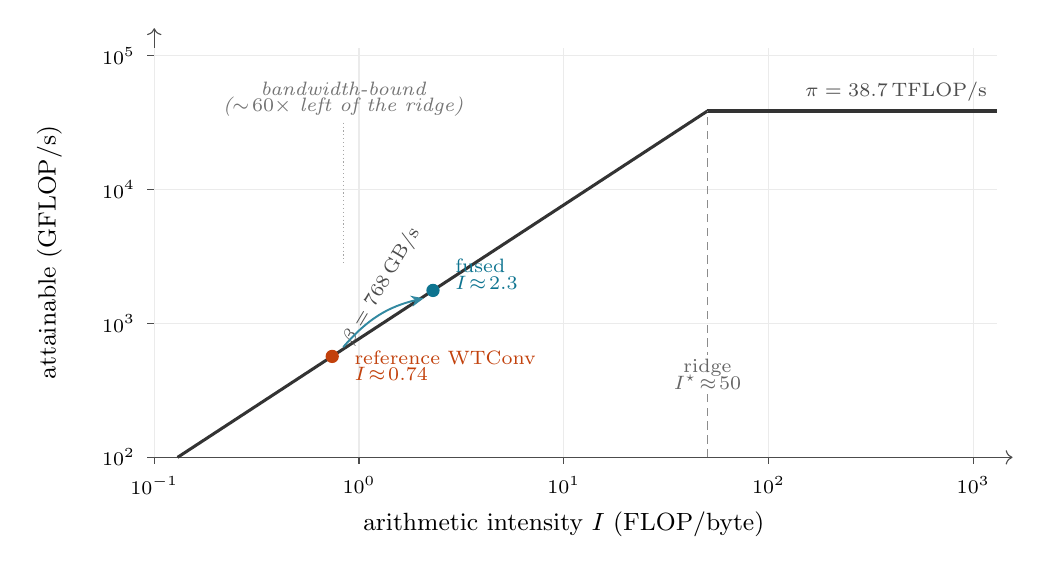
\begin{tikzpicture}[font=\small]

% ---------------------------------------------------------------- axes
\draw[->, black!70] (0,0) -- (10.9,0);
\node[font=\small] at (5.2,-0.85) {arithmetic intensity $I$ (FLOP/byte)};
\draw[->, black!70] (0,0) -- (0,5.45);
\node[rotate=90, anchor=south, font=\small] at (-1.05,2.6)
  {attainable (GFLOP/s)};

\foreach \x/\lab in {0/$10^{-1}$, 2.6/$10^{0}$, 5.2/$10^{1}$, 7.8/$10^{2}$, 10.4/$10^{3}$} {
  \draw[black!70] (\x,0) -- (\x,-0.09);
  \node[below, font=\scriptsize] at (\x,-0.12) {\lab};
}
\foreach \y/\lab in {0/$10^{2}$, 1.7/$10^{3}$, 3.4/$10^{4}$, 5.1/$10^{5}$} {
  \draw[black!70] (0,\y) -- (-0.09,\y);
  \node[left, font=\scriptsize] at (-0.12,\y) {\lab};
}
\foreach \x in {0,2.6,5.2,7.8,10.4} \draw[black!8] (\x,0) -- (\x,5.2);
\foreach \y in {1.7,3.4,5.1} \draw[black!8] (0,\y) -- (10.7,\y);

% ------------------------------------------------------- the roof itself
% bandwidth roof: P = beta*I, from I=0.13 (P=100) to the ridge at I=50.4
\draw[line width=1.1pt, black!80] (0.296,0) -- (7.026,4.399);
% compute ceiling: P = pi
\draw[line width=1.1pt, black!80] (7.026,4.399) -- (10.7,4.399);
\node[above left, font=\scriptsize, text=black!70] at (10.7,4.40)
  {$\pi=38.7$\,TFLOP/s};
\node[font=\scriptsize, text=black!70, rotate=59, anchor=south] at (3.1,2.05)
  {$\beta=768$\,GB/s};

% ridge marker
\draw[densely dashed, black!45] (7.026,0) -- (7.026,4.399);
\node[font=\scriptsize, text=black!60, align=center, fill=white, inner sep=1.5pt]
  at (7.026,1.05) {ridge\\[-2pt]$I^\star\!\approx\!50$};

% --------------------------------------------------- the two measured points
% reference: I = 0.74 -> 568 GFLOP/s
\fill[hbmcol] (2.260,1.282) circle (2.4pt);
\node[anchor=west, font=\scriptsize, text=hbmcol, align=left]
  at (2.42,1.16) {reference WTConv\\[-2pt]$I\!\approx\!0.74$};

% fused: I = 2.3 -> 1766 GFLOP/s
\fill[regcol] (3.540,2.120) circle (2.4pt);
\node[anchor=west, font=\scriptsize, text=regcol, align=left]
  at (3.70,2.32) {fused\\[-2pt]$I\!\approx\!2.3$};

% the move
\draw[-{Stealth[length=4.5pt,width=4pt]}, regcol!85, line width=0.7pt]
  (2.40,1.40) to[bend left=18] (3.42,2.02);

% shaded bandwidth-bound region annotation
\node[font=\scriptsize\itshape, text=black!55, align=center] at (2.4,4.55)
  {bandwidth-bound\\[-2pt]($\sim\!60\times$ left of the ridge)};
\draw[densely dotted, black!35] (2.4,4.25) -- (2.4,2.45);

\end{tikzpicture}

\caption{Roofline for the RTX~A6000 ($\beta=768$\,GB/s, $\pi=38.7$\,TFLOP/s in \texttt{fp32}, ridge at $I^\star\approx50$\,FLOP/byte). The reference WTConv layer sits at $I\approx0.74$\,FLOP/byte and the fused formulation at $I\approx2.3$\,FLOP/byte. Both are far inside the bandwidth-limited region, which is why traffic rather than arithmetic is the quantity worth minimising; it is not a claim that latency is proportional to it (\Cref{sec:prediction}). Fusion does not move the operator across the ridge; it moves it \emph{up the bandwidth roof} by raising the work done per byte.}
\label{fig:roofline}
\end{figure}

%==============================================================================
\section{Realisation}
\label{sec:implementation}
%==============================================================================

We realise \Cref{eq:qfused} as three CUDA kernels in the forward direction (one at $L{=}1$) plus the folded base convolution. The whole wavelet branch is exposed as a single \texttt{torch.autograd.Function} matching the reference module's interface, so the layer is a drop-in replacement; owning the branch as one node is also what lets the raw-low-pass gradient fold into the same kernel as the coefficient gradients, rather than arriving as a separate full-resolution tensor to be added.

\paragraph{Analysis kernel.} One thread produces the four subband outputs at one coefficient position, looping over the $k^2$ taps and holding four \texttt{fp32} accumulators in registers. A block stages the Haar partial sums for its output tile, plus a $k-1$ halo, in shared memory, so each input element is fetched once per tile instead of once per tap; $k$ is a template parameter, so the tap loops are fully unrolled. This kernel runs once per level $\ell\ge2$. Level~1 instead runs the collapsed kernel below, and its raw low-pass band comes from a small preceding pass.

\paragraph{Collapsed level kernel.} At level~1 one thread stages partial sums, runs the same tap loop, adds the deeper levels' reconstruction into its low-pass accumulator, applies the inverse butterfly of \Cref{sec:levelcollapse} in registers, adds the base-path output and stores its $2\times2$ block once. Neither the coefficient tensor nor a separate reconstruction is ever written.

\paragraph{Synthesis kernel.} One thread evaluates \Cref{prop:bitindexed} across levels $2,\dots,L$ by shift-and-parity addressing, writing one value onto level~1's coefficient grid. At $L{=}1$ it does not run at all.

\paragraph{Backward.} Because $\mH$ is self-inverse, the gradient of the collapsed level is the same tap loop driven by the Haar coefficients of the output gradient, and each thread writes a disjoint $2\times2$ input-gradient block, so the scatter needs no atomics. The weight gradient is the same reduction with the roles of "sum over taps" and "sum over positions" exchanged, $\partial\mathcal{L}/\partial\widetilde{\mW}_s[\kappa_h,\kappa_w] = \sum_{b,h',w'} \partial\mathcal{L}/\partial\tZ_s[h',w']\cdot P_s\bigl(h'+\kappa_h-\tfrac{k-1}{2},\,w'+\kappa_w-\tfrac{k-1}{2}\bigr)$; recomputing the partial sums $P_s$ in shared memory means the coefficients are not materialised in the backward pass either, which replaces the grouped depthwise weight gradient that otherwise dominates a training step. Accumulation across blocks uses \texttt{fp32} atomics, so this gradient is not bitwise reproducible across runs, as the vendor's is not.

\paragraph{Precision.} \texttt{fp32}, \texttt{fp16} and \texttt{bf16} inputs are supported; all butterflies, tap accumulations and cross-level sums are performed in \texttt{fp32} and rounded once at the store. Since the operator is bandwidth-bound, reduced precision halves the traffic and therefore roughly halves the runtime; reduced precision is a bandwidth optimisation here, not an arithmetic one.

\paragraph{Scope.} The kernels implement Haar (\texttt{db1}) only, depthwise with $C_{\mathrm{in}}=C_{\mathrm{out}}$, odd $k$, and $L\le5$; these match the configurations the reference layer is used in, but they are genuine restrictions and we return to them in \Cref{sec:limitations}.

%==============================================================================
\section{Experiments}
\label{sec:experiments}
%==============================================================================

\subsection{Setup}

All measurements are single-layer microbenchmarks on one NVIDIA RTX~A6000 unless stated otherwise. We sweep $C\in\{32,64,128\}$, $H=W\in\{128,256,512\}$ at batch size $8$, and $L\in\{1,\dots,5\}$, with $k=3$. Latency is measured with CUDA events over $50$ timed iterations after $20$ warmup iterations, which absorb JIT compilation, autotuning and cuDNN algorithm selection; peak memory is \texttt{torch.cuda.max\_memory\_allocated} after \texttt{reset\_peak\_memory\_stats}. Reported ratios are geometric means over the $(C,H)$ sweep. Two protocols are used: \emph{homogeneous}, where every method uses $k=3$, isolating the cost of the wavelet machinery; and \emph{receptive-field-matched}, where WTConv at $k=3$ is compared against plain convolutions at $k=7$, which is the substitution the layer is actually proposed for. Neither arm uses \texttt{torch.compile}; see \Cref{sec:limitations}.

\subsection{Numerical equivalence}
\label{sec:equivalence}

Every step in \Cref{sec:method} is an algebraic identity, so the fused layer and the reference compute the same function and should differ only by floating-point reassociation. We test this directly: weights are copied from a reference module into the fused module, both are driven with the same input and the same random cotangent, and we compare the forward output and every gradient the layer produces: $\nabla_{\!X}$, $\nabla_{\!W}$ for the base and all $L$ wavelet levels, and $\nabla_{\!s}$ for all scales. We additionally verify the two structural claims the derivation rests on rather than assuming them: that $\mH=\mH^{\!\top}=\mH^{-1}$ exactly (\Cref{prop:selfinverse}), and that the reference's subband packing matches the ordering the fused kernels assume. \Cref{tab:correctness} reports the results. Testing the gradients, rather than the forward pass alone, is what exposed the scale-fold error of \Cref{eq:foldgrad}: the forward pass agreed to machine precision throughout while $\nabla_{\!W}$ was wrong by a per-channel factor.

% Generated by scripts/make_tables.py -- do not edit by hand.
% Regenerate with:  python make_tables.py --bench ... --correctness ...

\begin{table}[t]
\centering
\caption{Numerical agreement with the reference implementation. Entries are maximum absolute deviation over the whole tensor, at $L$ decomposition levels, for the forward output and input gradient. The fused kernels compute the same multilinear map with a different association order, so the residual is floating-point reassociation error alone.}
\label{tab:correctness}
\begin{tabular}{llccc}
\toprule
Backend & dtype & $L$ & forward & $\nabla_X$ \\
\midrule
Fused (CUDA) & \texttt{fp32} & 1 & 2.4e-07 & 2.4e-07 \\
Fused (CUDA) & \texttt{fp32} & 2 & 2.4e-07 & 2.4e-07 \\
Fused (CUDA) & \texttt{fp32} & 3 & 2.4e-07 & 2.4e-07 \\
Fused (CUDA) & \texttt{fp32} & 4 & 2.4e-07 & 2.4e-07 \\
Fused (CUDA) & \texttt{fp32} & 5 & 2.4e-07 & 2.4e-07 \\
\addlinespace[2pt]
Fused (CUDA) & \texttt{fp16} & 1 & 2.0e-03 & 9.8e-04 \\
Fused (CUDA) & \texttt{fp16} & 2 & 2.0e-03 & 2.0e-03 \\
Fused (CUDA) & \texttt{fp16} & 3 & 2.0e-03 & 2.0e-03 \\
Fused (CUDA) & \texttt{fp16} & 4 & 2.0e-03 & 2.0e-03 \\
Fused (CUDA) & \texttt{fp16} & 5 & 2.0e-03 & 2.0e-03 \\
\addlinespace[2pt]
Fused (CUDA) & \texttt{bf16} & 1 & 1.6e-02 & 1.6e-02 \\
Fused (CUDA) & \texttt{bf16} & 2 & 1.6e-02 & 1.6e-02 \\
Fused (CUDA) & \texttt{bf16} & 3 & 1.6e-02 & 7.8e-03 \\
Fused (CUDA) & \texttt{bf16} & 4 & 1.6e-02 & 1.6e-02 \\
Fused (CUDA) & \texttt{bf16} & 5 & 1.6e-02 & 1.6e-02 \\
\bottomrule
\end{tabular}
\end{table}

\subsection{Measured speedup}
\label{sec:speed}

% TODO(measurement): the numbers below predate the level-collapse of
% Sec.~\ref{sec:levelcollapse} and the fused weight gradient. Regenerate with
%   python scripts/bench.py --out results/raw.json && python scripts/make_tables.py
% before submission.
% Generated by scripts/seed_from_report.py from the authors' original
% measurement campaign. Re-running scripts/bench.py followed by
% scripts/make_tables.py regenerates this file from fresh measurements.
\begin{table}[t]
\centering
\caption{Forward latency of every method relative to the reference WTConv ($1.00\times$; higher is faster), all at $k{=}3$, CUDA backend on an RTX~A6000. Fusion recovers most---but not all---of the gap to a plain depthwise convolution, which is the honest statement of what the layer now costs.}
\label{tab:context}
\begin{tabular}{llccccc}
\toprule
\multirow{2}{*}{Method} & \multirow{2}{*}{Precision} & \multicolumn{5}{c}{Decomposition levels $L$} \\
\cmidrule(lr){3-7}
 & & 1 & 2 & 3 & 4 & 5 \\
\midrule
Depthwise conv, $k{=}3$ & \texttt{fp32} & 7.72$\times$ & 10.07$\times$ & 10.85$\times$ & 10.96$\times$ & 11.48$\times$ \\
 & \texttt{fp16} & 9.65$\times$ & 12.59$\times$ & 13.54$\times$ & 13.68$\times$ & 14.22$\times$ \\
\addlinespace[2pt]
Dense conv, $k{=}3$ & \texttt{fp32} & 3.86$\times$ & 5.04$\times$ & 5.42$\times$ & 5.48$\times$ & 5.63$\times$ \\
 & \texttt{fp16} & 3.65$\times$ & 4.74$\times$ & 5.05$\times$ & 5.25$\times$ & 5.41$\times$ \\
\addlinespace[2pt]
WTConv, reference & \texttt{fp32} & 1.00$\times$ & 1.00$\times$ & 1.00$\times$ & 1.00$\times$ & 1.00$\times$ \\
 & \texttt{fp16} & 1.00$\times$ & 1.00$\times$ & 1.00$\times$ & 1.00$\times$ & 1.00$\times$ \\
\addlinespace[2pt]
WTConv, \textbf{fused} & \texttt{fp32} & 2.24$\times$ & 2.72$\times$ & 2.82$\times$ & 2.85$\times$ & 2.87$\times$ \\
 & \texttt{fp16} & 2.99$\times$ & 3.65$\times$ & 3.79$\times$ & 3.83$\times$ & 3.84$\times$ \\
\addlinespace[2pt]
\bottomrule
\end{tabular}
\end{table}


\Cref{tab:context} reports measured forward latency for every method relative to the reference, and states the honest limit of what fusion buys. The fused layer is faster than the reference at every level and in both precisions, while remaining slower than a plain depthwise convolution at matched $k$ --- unsurprisingly, since it does $L$ times the work at geometrically decreasing resolution --- though it closes most of that gap. We report these as measurements rather than as confirmation of a predicted ratio. \Cref{tab:traffic} says the fused form moves $2.7$--$3.6\times$ fewer elements; that is the mechanism, but the two ratios are different quantities and we do not expect them to coincide (\Cref{sec:prediction}).

One observation does bear on the mechanism. The \texttt{fp16} ratios exceed the \texttt{fp32} ones throughout, whereas halving the bytes halves the traffic on both sides and would leave a pure bandwidth account unchanged. The excess is therefore not explained by the element counts of \Cref{sec:prediction}, and we do not claim it is; it indicates that the reference path incurs precision-conversion traffic that our accounting does not model.

\Cref{tab:memory} reports peak memory, where the reference needs $1.46$--$1.50\times$ more; this is nearly flat in $L$ because the dominant saved allocation is the level-1 coefficient tensor, which is four times larger than all deeper levels combined and which \Cref{sec:levelcollapse} removes outright.

% Generated by scripts/make_tables.py -- do not edit by hand.
% Regenerate with:  python make_tables.py --bench ... --correctness ...

\begin{table}[t]
\centering
\caption{Peak allocated memory over a training step relative to the reference WTConv ($1.00\times$; higher means the method needs less memory), same sweep as \Cref{tab:latency}. Measured as the CUDA allocator high-water mark, not reserved memory. Fusion removes the per-level coefficient tensors from the autograd tape, which is where the saving comes from.}
\label{tab:memory}
\begin{tabular}{llccccc}
\toprule
\multirow{2}{*}{Method} & \multirow{2}{*}{Precision} & \multicolumn{5}{c}{Decomposition levels $L$} \\
\cmidrule(lr){3-7}
 & & 1 & 2 & 3 & 4 & 5 \\
\midrule
Depthwise conv, $k{=}3$ & \texttt{fp32} & 1.59$\times$ & 2.32$\times$ & 2.32$\times$ & 2.32$\times$ & 2.32$\times$ \\
 & \texttt{fp16} & 1.38$\times$ & 2.01$\times$ & 2.01$\times$ & 2.01$\times$ & 2.01$\times$ \\
\addlinespace[2pt]
Dense conv, $k{=}3$ & \texttt{fp32} & 1.60$\times$ & 2.33$\times$ & 2.33$\times$ & 2.33$\times$ & 2.33$\times$ \\
 & \texttt{fp16} & 1.52$\times$ & 2.22$\times$ & 2.22$\times$ & 2.22$\times$ & 2.22$\times$ \\
\addlinespace[2pt]
Depthwise conv, $k{=}7$ & \texttt{fp32} & 1.59$\times$ & 2.32$\times$ & 2.32$\times$ & 2.32$\times$ & 2.32$\times$ \\
 & \texttt{fp16} & 1.38$\times$ & 2.01$\times$ & 2.01$\times$ & 2.01$\times$ & 2.01$\times$ \\
\addlinespace[2pt]
Dense conv, $k{=}7$ & \texttt{fp32} & 1.51$\times$ & 2.19$\times$ & 2.19$\times$ & 2.19$\times$ & 2.19$\times$ \\
 & \texttt{fp16} & 1.48$\times$ & 2.15$\times$ & 2.15$\times$ & 2.15$\times$ & 2.15$\times$ \\
\addlinespace[2pt]
WTConv, reference & \texttt{fp32} & 1.00$\times$ & 1.00$\times$ & 1.00$\times$ & 1.00$\times$ & 1.00$\times$ \\
 & \texttt{fp16} & 1.00$\times$ & 1.00$\times$ & 1.00$\times$ & 1.00$\times$ & 1.00$\times$ \\
\addlinespace[2pt]
WTConv, \textbf{fused} & \texttt{fp32} & 1.85$\times$ & 2.34$\times$ & 2.29$\times$ & 2.28$\times$ & 2.28$\times$ \\
 & \texttt{fp16} & 1.85$\times$ & 2.34$\times$ & 2.29$\times$ & 2.28$\times$ & 2.27$\times$ \\
\addlinespace[2pt]
\bottomrule
\end{tabular}
\end{table}


The receptive-field-matched comparison (\Cref{app:rfmatch}) is the one that reflects intended use: against a dense $7\times7$ convolution, the reference WTConv is $1.14$--$1.65\times$ \emph{slower} in \texttt{fp32}, whereas the fused layer is $1.75$--$1.96\times$ \emph{faster} at every level. This reverses the practical verdict on the operator.

\subsection{Training parity}

Numerical equivalence at a single step does not by itself establish that optimisation behaves identically over a long run. We train a MobileNetV2-style network with WTConv replacing the depthwise convolutions on CIFAR-10 at $256\times256$ (SGD, momentum $0.9$, learning rate $0.01$, batch size $32$, 50 epochs, NVIDIA L40S), with the reference and fused layers initialised from identical weights. Training loss curves are indistinguishable and final validation accuracy matches to within run-to-run noise, at $2.55\times$ end-to-end training throughput (\Cref{fig:convergence}). We report this as a consistency check on a single run, not as an accuracy claim: it has no seed replicates, and it inherits the caveats in \Cref{sec:limitations}.

\begin{figure}[t]
\centering
% Convergence panels, cropped from the Weights & Biases export of the
% CIFAR-10 / WTMobileNet run (figures/wandb.pdf).
% Card bounding boxes measured at 72 dpi (1 px = 1 pt) on the 595x842 pages:
%   p1 validation accuracy : x 124..470, y 366..668
%   p2 throughput ratio    : x 124..470, y  37..375
%   p2 training loss       : x 124..470, y 378..677
% trim = {left, bottom, right, top} removed, in pt.
\begin{tikzpicture}[node distance=2mm]
  \node (a)
    {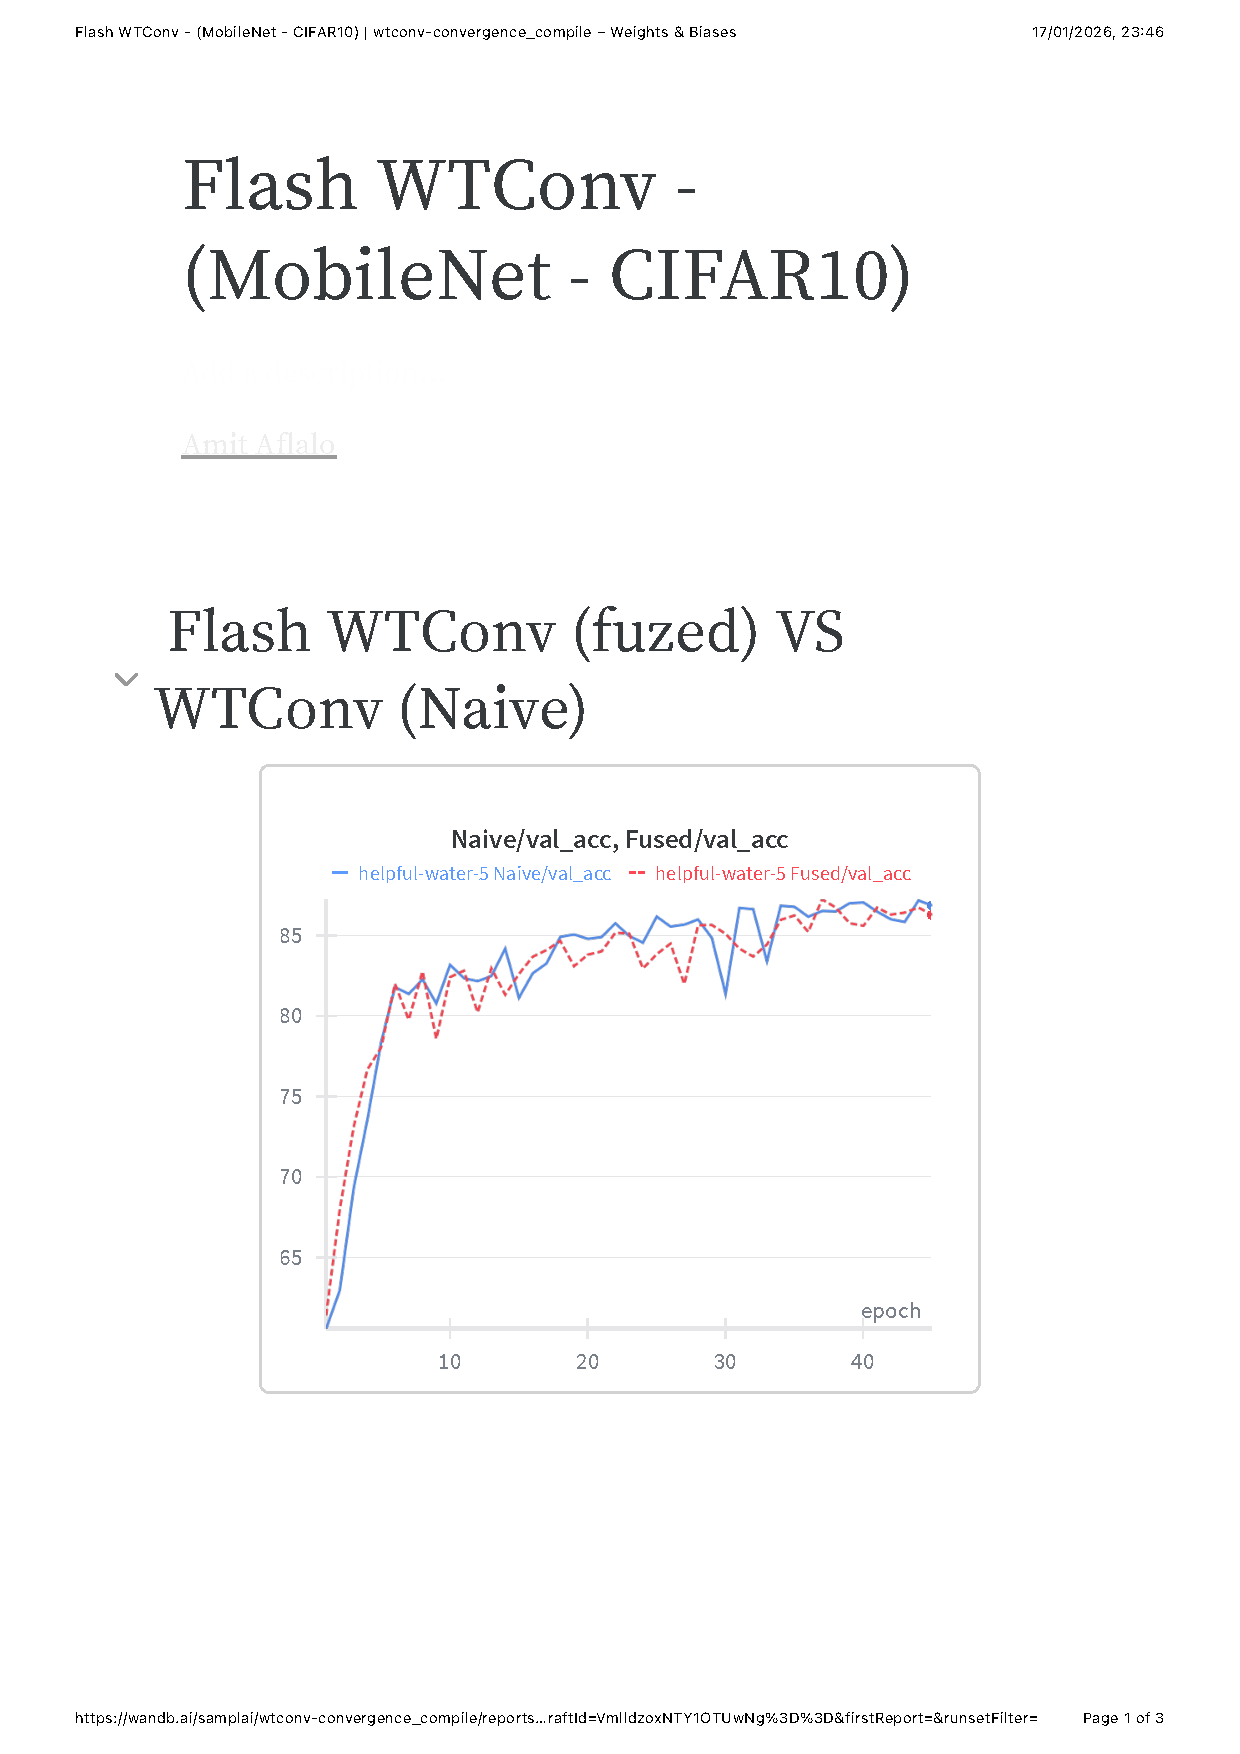
\includegraphics[height=4.1cm, page=1,
       trim=124pt 174pt 125pt 366pt, clip]{figures/wandb.pdf}};
  \node[right=of a] (b)
    {\includegraphics[height=4.1cm, page=2,
       trim=124pt 165pt 125pt 378pt, clip]{figures/wandb.pdf}};
  \node[right=of b] (c)
    {\includegraphics[height=4.1cm, page=2,
       trim=124pt 467pt 125pt 37pt, clip]{figures/wandb.pdf}};
  \node[below=0.8mm of a, font=\scriptsize] {(a) validation accuracy};
  \node[below=0.8mm of b, font=\scriptsize] {(b) training loss};
  \node[below=0.8mm of c, font=\scriptsize] {(c) throughput ratio};
\end{tikzpicture}

\caption{Training a MobileNetV2-style backbone with WTConv depthwise layers on CIFAR-10 at $256\times256$ for 50 epochs, reference against fused, from identical initial weights. Validation accuracy (a) and training loss (b) are indistinguishable, while the fused layer sustains $2.55\times$ the training throughput (c). This is a single run and is reported as a consistency check on the equivalence argument, not as an accuracy result.}
\label{fig:convergence}
\end{figure}

%==============================================================================
\section{Portability}
\label{sec:portability}
%==============================================================================

The reformulation of \Cref{sec:method} appeals only to the algebra of the Haar basis and to the existence of a memory hierarchy. It uses no CUDA-specific feature (no warp primitive, no tensor core, no architecture intrinsic), so it should transfer to any accelerator whose cost is dominated by traffic to a large, slow memory. We tested this by re-deriving the same kernels twice more.

A Triton \citep{tillet2019triton} realisation expresses the register-resident analysis and the bit-indexed synthesis directly, with block size and warp count left to autotuning; it matches or slightly exceeds the CUDA realisation in \texttt{fp32} ($2.71$--$3.09\times$) and is marginally behind in \texttt{fp16}. An Apple Metal realisation on an M3~Pro, benchmarked against PyTorch's MPS backend, reaches $2.05$--$2.40\times$. That the same three identities produce comparable ratios on three unrelated software stacks and two unrelated hardware vendors is the strongest evidence we have that the mechanism is the I/O account rather than any platform-specific tuning. Full tables, and the caveats specific to each backend (in particular that the Metal comparison is against a substantially less mature vendor baseline than cuDNN, which inflates the Apple-side numbers), are in \Cref{app:backends}.

%==============================================================================
\section{Related work}
\label{sec:related}
%==============================================================================

\paragraph{Large receptive fields in CNNs.} The effective receptive field of a deep CNN grows only as $\mathcal{O}(\sqrt{n})$ in depth \citep{luo2016erf}, motivating dilation \citep{yu2016dilated} and directly enlarged kernels \citep{ding2022replknet,liu2023slak}, which pay in parameters and FLOPs. WTConv \citep{finder2024wavelet} instead makes parameters logarithmic in the receptive field. This literature optimises parameters and FLOPs; our point is that for WTConv neither quantity is what determines runtime.

\paragraph{Wavelets in deep learning.} Multiresolution analysis and the filter-bank algorithm \citep{mallat1989multiresolution} on the Haar basis \citep{haar1910} underpin a line of work using the DWT as an aliasing-free replacement for pooling and downsampling \citep{williams2018waveletpooling,li2020wavecnet} and as a multi-scale backbone for restoration \citep{liu2018mwcnn}. All of these invoke the transform through a framework \texttt{conv2d}, treating it as a fixed primitive. We treat it instead as a fusion boundary to be dissolved.

\paragraph{Fast wavelet transforms.} The lifting scheme factors a wavelet transform into in-place prediction and update steps \citep{sweldens1996lifting,sweldens1998lifting,daubechies1998factoring}, reducing operation count and enabling in-place evaluation; GPU implementations have long compared filter-bank against lifting formulations \citep{tenllado2008dwtgpu}. That literature optimises the transform in isolation. The transform is not the bottleneck here: our gain comes from fusing it into the surrounding convolution so that it never touches memory at all, and for Haar specifically the lifting factorisation coincides with the butterfly of \Cref{eq:butterfly}.

\paragraph{Kernel fusion and memory-bound operators.} That data movement rather than arithmetic limits deep learning is well established \citep{ivanov2021datamovement,wahib2014kernelfusion}, and FlashAttention \citep{dao2022flashattention,dao2024flashattention2} is the canonical demonstration that an exact reassociation which keeps intermediates on chip can transform an operator's practical cost. Our work is the same argument applied to a different operator, with the additional structure that the transform being fused is multiplication-free, symmetric, and self-inverse. These properties make recomputation inexpensive and let analysis and synthesis exchange roles during backpropagation. General-purpose compilers \citep{ragankelley2013halide,chen2018tvm,sabne2020xla,ansel2024pytorch2} automate fusion of elementwise and reduction chains, but the reassociations of \Cref{sec:synthesis}, collapsing an $L$-step recursion into a closed-form bit-indexed sum, rest on properties of the Haar basis that a general compiler does not have access to.

\paragraph{Depthwise convolution efficiency.} Depthwise convolutions have low arithmetic intensity and are known to underutilise GPUs relative to their FLOP count \citep{howard2017mobilenets,ma2018shufflenetv2,lu2022depthwisegpu}. WTConv inherits this and compounds it with a per-level chain of full-tensor intermediates.

%==============================================================================
\section{Limitations}
\label{sec:limitations}
%==============================================================================

\textbf{Scope of the kernels.} They implement Haar (\texttt{db1}) only. The reference layer accepts any PyWavelets family, and a model trained with \texttt{db2} or longer cannot use our kernels. The multiplication-free argument of \Cref{sec:analysis} is specific to Haar; longer filters would still admit the reformulation but with a materially worse recompute trade. We also require depthwise operation with $C_{\mathrm{in}}=C_{\mathrm{out}}$, odd $k$, and $L\le5$ (the last is a hand-unrolled dispatch limit, not an algorithmic one).

\textbf{Compilation.} All results are eager-mode on both arms. Our layer opts out of Dynamo tracing, so we cannot report a fair \texttt{torch.compile} comparison; an inductor-generated fusion of the reference is a baseline this paper does not measure, and a reviewer is right to want it. We expect inductor to fuse the elementwise scale but not to discover \Cref{prop:bitindexed}.

\textbf{Measurement.} Single-layer microbenchmarks on one GPU per platform, with a fixed resident input tensor and no host-to-device transfer. We report geometric means over the configuration sweep and per-iteration dispersion, but no cross-machine replication. The end-to-end training result is a single run without seed replicates, and Amdahl's law applies: a $2.5\times$ layer speedup yields a smaller whole-model speedup, which is why we report the measured $2.55\times$ end-to-end training throughput rather than extrapolating from the layer numbers.

\textbf{Shift-variance.} As is already true of the reference operator, the $2^{\ell}$-aligned decomposition grid makes WTConv equivariant only to translations by multiples of $2^{L}$. Our reformulation is exactly equivalent, so it neither introduces nor removes this property.

\textbf{Backend maturity.} The Metal comparison is against PyTorch's MPS backend, which is considerably less mature than cuDNN; the Apple-side ratios should be read as a portability demonstration, not as a like-for-like vendor comparison.

%==============================================================================
\section{Conclusion}
%==============================================================================

WTConv's difficulty was never its arithmetic. Expressed as a chain of framework primitives it runs at under $2\%$ of a modern GPU's arithmetic capability, spending its time moving tensors that need never have existed. Accounting for those bytes exactly, and removing them with four algebraic identities (a register-resident multiplication-free analysis, a synthesis cascade collapsed into a bit-indexed closed form, a finest level collapsed end to end into a polyphase convolution, and a scale folded into the weights), yields a bit-exact reformulation whose cost is within a small constant of the compulsory traffic. We do not claim that the ratio of bytes predicts the ratio of seconds; what the account buys is the identification of the quantity to remove, and that the same identities reproduce the gain on two other stacks suggests the identification is the right one. The broader point is that an operator's asymptotic parameter or FLOP advantage says little about whether it is usable; for the growing class of layers built from cheap, structured, multi-stage transforms, the I/O cost model is the one that predicts practice.

\subsubsection*{Broader Impact Statement}
This work reduces the time and energy required to evaluate an existing operator without changing its function; the primary effect is lower computational cost for practitioners already using WTConv. We see no application-specific ethical concerns beyond those already attached to efficient computer vision generally.

\bibliography{main}
\bibliographystyle{tmlr}

\appendix

\section{Reproducibility}
\label{app:repro}

\subsection{Measurement protocol}

\paragraph{End-to-end architecture.}
All three end-to-end models are untrained, 1,000-class Tiny variants with a
$4\times4$, stride-4 patch stem; output stride 32; four stages with block depths
$(3,3,9,3)$ and channel widths $(96,192,384,768)$; and a global-average-pooling,
LayerNorm, linear classification head. Blocks use GELU, layer-scale
initialization $10^{-6}$, no convolutional MLP or global response normalization,
and zero dropout and stochastic-depth rates. ConvNeXt-T uses a $7\times7$
depthwise convolution in each block. Both WTConvNeXt-T variants replace it with
$5\times5$ WTConv at stage-wise decomposition levels $(5,4,3,2)$ and differ
only in whether WTConv uses the reference or fused implementation. Measurements
use FP32 inputs of shape $(64,3,224,224)$.

\paragraph{Timing.}
For each layer configuration and end-to-end model, we run $20$ untimed warm-up
iterations followed by $50$ measured iterations. Warm-up excludes first-use
compilation and cuDNN setup. We synchronize CUDA before and after the measured
loop and use CUDA events to record each iteration's device time. Layerwise
benchmarks run eagerly: inference measures a forward pass without gradients,
whereas forward--backward timing includes an output reduction, backpropagation,
and gradient clearing, but no task loss or optimizer update. End-to-end models
use \verb|torch.compile| uniformly. Their training step includes gradient
clearing, a forward pass with cross-entropy loss, backpropagation, and an SGD
update. All inputs and targets are GPU-resident, so data loading and host-to-device
transfers are excluded.

\paragraph{Memory.} \verb|torch.cuda.reset_peak_memory_stats| followed by one
untimed step and \verb|torch.cuda.max_memory_allocated|. This measures
allocator high-water mark, not reserved memory.


\subsection{Environment}

primary measurements used an NVIDIA RTX A6000 (compute capability 8.6, 47.5 GiB), Python 3.12.12, PyTorch 2.6.0+cu124, CUDA 12.4, cuDNN 9.1.0, driver 550.163.01, nvcc 12.4.99, and GCC/G++ 11.4.0. The cross-hardware sweep used an NVIDIA RTX PRO 6000 Blackwell Max-Q (compute capability 12.0, 95.0 GiB), Python 3.12.12, PyTorch 2.9.1+cu130, CUDA 13.0, and cuDNN 9.13.0, driver 595.71.05, nvcc 13.0, and GCC/G++ 11.4.0.


\section{Receptive-field-matched comparison}
\label{app:rfmatch}

\Cref{tab:context} compares every method at the same kernel size, which isolates
the cost of the wavelet machinery but is not the comparison a practitioner faces.
WTConv is proposed as a replacement for a \emph{large} convolution: an $L$-level
layer at $k{=}3$ reaches $3\cdot2^{L}$ pixels, so even $L{=}2$ already exceeds the
footprint of a $7\times7$ kernel. \Cref{tab:rfmatch} therefore repeats the
measurement with the plain-convolution baselines at $k{=}7$, all ratios again
taken against the reference WTConv.

The comparison changes the verdict on the operator. Against a dense $7\times7$
convolution the reference WTConv is $1.14$--$1.65\times$ slower in \texttt{fp32},
so on wall-clock grounds it is the worse choice despite its parameter advantage;
the fused layer is $1.75$--$1.96\times$ faster than that same dense convolution
at every level. Against a depthwise $7\times7$ convolution, a much cheaper
baseline that does not mix channels, the fused layer is roughly at parity in
\texttt{fp32} and ahead in \texttt{fp16}. We report the depthwise column for
completeness rather than as the intended substitution, since a depthwise
$7\times7$ layer is not functionally interchangeable with a dense one.

% Generated by scripts/seed_from_report.py from the authors' original
% measurement campaign. Re-running scripts/bench.py followed by
% scripts/make_tables.py regenerates this file from fresh measurements.
\begin{table}[t]
\centering
\caption{Receptive-field-matched comparison: WTConv at $k{=}3$ against plain convolutions at $k{=}7$, all relative to the reference WTConv ($1.00\times$; higher is faster), CUDA backend on an RTX~A6000. The reference WTConv is \emph{slower} than the dense convolution it is meant to replace; the fused layer is faster than it at every level.}
\label{tab:rfmatch}
\begin{tabular}{llccccc}
\toprule
\multirow{2}{*}{Method} & \multirow{2}{*}{Precision} & \multicolumn{5}{c}{Decomposition levels $L$} \\
\cmidrule(lr){3-7}
 & & 1 & 2 & 3 & 4 & 5 \\
\midrule
Depthwise conv, $k{=}7$ & \texttt{fp32} & 2.07$\times$ & 2.72$\times$ & 2.89$\times$ & 2.96$\times$ & 3.01$\times$ \\
 & \texttt{fp16} & 1.39$\times$ & 1.82$\times$ & 1.94$\times$ & 2.03$\times$ & 2.06$\times$ \\
\addlinespace[2pt]
Dense conv, $k{=}7$ & \texttt{fp32} & 1.14$\times$ & 1.49$\times$ & 1.59$\times$ & 1.62$\times$ & 1.65$\times$ \\
 & \texttt{fp16} & 1.29$\times$ & 1.68$\times$ & 1.80$\times$ & 1.87$\times$ & 1.90$\times$ \\
\addlinespace[2pt]
WTConv, reference & \texttt{fp32} & 1.00$\times$ & 1.00$\times$ & 1.00$\times$ & 1.00$\times$ & 1.00$\times$ \\
 & \texttt{fp16} & 1.00$\times$ & 1.00$\times$ & 1.00$\times$ & 1.00$\times$ & 1.00$\times$ \\
\addlinespace[2pt]
WTConv, \textbf{fused} & \texttt{fp32} & 2.24$\times$ & 2.72$\times$ & 2.83$\times$ & 2.87$\times$ & 2.89$\times$ \\
 & \texttt{fp16} & 2.96$\times$ & 3.62$\times$ & 3.77$\times$ & 3.85$\times$ & 3.84$\times$ \\
\addlinespace[2pt]
\bottomrule
\end{tabular}
\end{table}


\section{Other backends}
\label{app:backends}
The reformulation of Section~\ref{sec:method} is stated in terms of algebra and
memory traffic, so it carries over to any accelerator whose cost is dominated by
traffic to a large, slow memory. We re-derived the same two kernels twice more
as a test of that claim. Table~\ref{tab:backends} collects the results.

% Generated by scripts/seed_from_report.py from the authors' original
% measurement campaign. Re-running scripts/bench.py followed by
% scripts/make_tables.py regenerates this file from fresh measurements.
\begin{table}[t]
\centering
\caption{Speedup over the reference implementation for all three realisations of the same reformulation, homogeneous protocol ($k{=}3$). The Metal figures are measured against PyTorch's MPS backend, which is markedly less mature than cuDNN; they demonstrate portability of the formulation rather than a like-for-like vendor comparison.}
\label{tab:backends}
\begin{tabular}{lllccccc}
\toprule
\multirow{2}{*}{Backend} & \multirow{2}{*}{Hardware} & \multirow{2}{*}{Precision} & \multicolumn{5}{c}{Decomposition levels $L$} \\
\cmidrule(lr){4-8}
 & & & 1 & 2 & 3 & 4 & 5 \\
\midrule
CUDA & RTX A6000 & \texttt{fp32} & 2.24$\times$ & 2.72$\times$ & 2.82$\times$ & 2.85$\times$ & 2.87$\times$ \\
 &  & \texttt{fp16} & 2.99$\times$ & 3.65$\times$ & 3.79$\times$ & 3.83$\times$ & 3.84$\times$ \\
\addlinespace[2pt]
Triton & RTX A6000 & \texttt{fp32} & 2.71$\times$ & 3.09$\times$ & 3.03$\times$ & 2.90$\times$ & 2.81$\times$ \\
 &  & \texttt{fp16} & 2.94$\times$ & 3.16$\times$ & 3.00$\times$ & 2.81$\times$ & 2.69$\times$ \\
\addlinespace[2pt]
Metal & M3 Pro & \texttt{fp32} & 2.05$\times$ & 2.34$\times$ & 2.40$\times$ & 2.37$\times$ & 2.31$\times$ \\
 &  & \texttt{fp16} & 2.05$\times$ & 2.13$\times$ & 2.20$\times$ & 2.20$\times$ & 2.15$\times$ \\
\addlinespace[2pt]
\bottomrule
\end{tabular}
\end{table}


\subsection{Triton}

The Triton realisation \citep{tillet2019triton} expresses the register-resident
analysis of Section~\ref{sec:method} directly: for each coefficient position the
kernel iterates the $k\times k$ tap grid with \verb|tl.static_range|, addresses
the corresponding $2\times2$ input block, forms the four subband values, and
accumulates into four \texttt{fp32} vectors. Because the kernel loads a compact
four-element weight vector per tap rather than an effective $(C,4,k,k)$ kernel
per output, its weight traffic is a quarter of the naive fused form. Block size,
warp count and pipeline depth are left to autotuning over eleven configurations
keyed on problem size.

The backward pass mirrors the forward: it iterates the same grid, applies the
transposed butterfly to the incoming subband gradients, and writes to a
\emph{disjoint} $2\times2$ input block per thread, so no atomics are required for
$\nabla_{\!X}$. Weight and scale gradients use Eq.~\eqref{eq:foldgrad} over
recomputed coefficients.

Performance matches the CUDA realisation closely --- slightly ahead in
\texttt{fp32} ($2.71$--$3.09\times$ against $2.24$--$2.89\times$) and slightly
behind in \texttt{fp16} --- which is the expected outcome if both are limited by
the same traffic. Two practical differences are worth recording. Triton's JIT
removes the dependency on a local \texttt{nvcc} installation, and its autotuner
adapts block sizes to the device without hand-tuning. Against that, the kernel
specialises on tensor shape, so a workload with many distinct shapes pays
repeated compilation, and the layer opts out of Dynamo tracing, so it cannot
currently be captured by \texttt{torch.compile}.

\subsection{Apple Metal}

The Metal realisation targets Apple Silicon through PyTorch's MPS backend. The
forward cascade uses a $16\times16$ threadgroup per $32\times32$ input tile,
staging the low-pass band in a single threadgroup buffer that is aliased and
overwritten in place at each level ($256\to64\to16\to4$ floats) with threads
retiring geometrically between barriers. The inverse cascade follows
Proposition~\ref{prop:bitindexed} per thread, exactly as in CUDA. As on NVIDIA,
\texttt{fp16} kernels convert to \texttt{fp32} on load, keep all butterflies and
all cross-level accumulation in \texttt{fp32}, and round once at the store; the
inter-level threadgroup buffer is \texttt{fp32} regardless of input precision.

Measured speedups are $2.05$--$2.40\times$. Three caveats attach to these
numbers and we would not want them read as a vendor comparison. First, the
baseline is PyTorch's generic MPS backend, which is substantially less mature
than cuDNN; this inflates the Apple-side ratios, and the dense-convolution
column in particular ($5\times$--$13\times$ slower than the fused layer) reflects
the maturity of the baseline far more than it reflects our kernels. Second, the
current dispatch issues a full stream synchronisation before encoding each
operation, which serialises host and device and makes these figures pessimistic
for end-to-end throughput on both arms. Third, several inverse dispatches
currently launch single-thread threadgroups, so occupancy is far below what the
formulation permits --- the Metal numbers should be read as a lower bound on
what the reformulation can deliver on this hardware rather than as a tuned
result.

\subsection{Coverage}

The CUDA and Triton paths support \texttt{fp32}, \texttt{fp16} and
\texttt{bf16}; the Metal path supports \texttt{fp32} and \texttt{fp16} only. All
three implement Haar with $L\le5$, depthwise, $C_{\mathrm{in}}=C_{\mathrm{out}}$,
and odd $k$.


\end{document}
